\documentclass[11pt]{article}

\usepackage[utf8]{inputenc}
\usepackage[T1]{fontenc}
\usepackage[margin=1.1in]{geometry}
\usepackage{booktabs}
\usepackage{graphicx}
\usepackage{amsmath}
\usepackage{siunitx}
\usepackage{microtype}
\usepackage[numbers,sort&compress]{natbib}
\usepackage{caption}
\usepackage[hidelinks]{hyperref}
\providecommand{\doi}[1]{\href{https://doi.org/#1}{doi:#1}}

\captionsetup{font=small,labelfont=bf}
\sisetup{detect-weight=true,detect-family=true}
\newcommand{\gap}{P\,$-$\,B}
\renewcommand{\arraystretch}{1.15}

\title{\bfseries Same probe, different depths:\\[3pt]
\large how the gap between output and internals scales\\[1pt]
in biological foundation models}

\author{%
  Ihor Kendiukhov\thanks{Correspondence:
  \texttt{ihor.kendiukhov@student.uni-tuebingen.de}}\\[2pt]
  \normalsize Institute of Medical Genetics and Applied Genomics,\\
  \normalsize University of T\"ubingen, T\"ubingen, Germany\\[2pt]
  \normalsize Pivotal Research
}
\date{22 August 2026}

\begin{document}
\maketitle

\begin{abstract}
\noindent
A language model can hold information internally that its outputs do not
express. For biological foundation models --- protein and genome language models
now used in enzyme design and variant effect prediction --- the size of that
discrepancy bears on whether output-only evaluation is a sufficient safety
practice. We define an \textbf{elicitation gap}: the difference between what a
model's sanctioned output expresses and what a linear readout recovers from its
best internal layer, both read at \emph{identical capacity}, so that a difference
is a property of the model rather than of the probe. We measure how it scales
across five tasks, two modalities and four model families, repeating every
experiment up to six times.

The gap widens with scale on some tasks and not others: clearly on fold
recognition ($+0.020$ per decade of parameters, 95\% CI $[+0.009, +0.031]$) and
enzyme function ($+0.021$, $[+0.014, +0.029]$); not detectably on two
ceiling-compressed transcription-factor tasks; and in the opposite direction on a
genome task ($-0.019$, $[-0.037, -0.001]$). Using a measurement that holds the
score fixed and varies the budget, we further find that the budget required to
reach a fixed capability falls with scale ($-0.118$ decades of budget per decade
of parameters, $[-0.181, -0.055]$).

Our central methodological finding is that single-run scaling claims in this
literature are unreliable in both directions. Our own headline reversed under
replication: one run gave ``no measurable change'' ($+0.018$, $[-0.011,
+0.046]$); six runs gave a clear widening ($+0.020$, $[+0.009, +0.031]$). The
point estimate barely moved --- only the interval did. Of twenty-nine measurement
defects we found in our own pipeline, every one of the twenty-six that biased a
number biased it in our favour, an asymmetry we argue is structural rather than
incidental.
\end{abstract}

\section{Introduction}

As models get larger, does the gap between what they say and what they internally
represent widen or close?

If it closes, output-only assessment becomes progressively safer as the field
advances: what you see is increasingly what the model has. If it widens,
output-only assessment becomes progressively \emph{more} misleading exactly as
models become more capable --- and for biological models the capability in
question includes designing enzymes, predicting variant effects, and reasoning
about viral fitness.

The question is not whether internal states contain more than outputs. For
protein models that is established: structural and functional information emerges
inside representations as pretraining scales~\citep{rives2021esm1b}, the best
internal layer outperforms the final layer on downstream tasks, with the deepest
layer winning in only 17.92\% of
model--task pairs across 13 protein language models and 15
tasks~\citep{joeres2026taskspecific}, and medium-sized models transferring as
well as large ones on realistic datasets~\citep{vieira2025medium}. The question
is whether that discrepancy is a fixed property of the architecture or a function
of scale, and that requires measuring it the same way across a ladder of model
sizes. We report slopes per decade of parameters, following the convention of the
scaling-law literature~\citep{kaplan2020scaling}, while measuring a different
quantity: not loss against scale, but the difference between two ways of reading
one model.

A second concern runs through this paper. Seed and split variance in
machine-learning benchmarks is large enough that single-run comparisons routinely
mistake noise for effect~\citep{bouthillier2021variance}, reported orderings can
reverse under reseeding alone~\citep{henderson2018deeprl}, and fine-tuned scores
vary substantially with initialisation and data order~\citep{dodge2020finetuning}.
We therefore repeat every measurement and report
intervals~\citep{miller2024errorbars}.

\subsection{Related work}

\paragraph{Capability elicitation.} That behavioural evaluation understates what a
model can do is established outside biology. Password-locked models show that
fine-tuning recovers capabilities that prompting does
not~\citep{greenblatt2024passwordlocked}; a direct comparison of prompting,
activation steering and fine-tuning concludes that fine-tuning should be the
method of choice for trustworthy capability
evaluation~\citep{hofstatter2025elicitation}; and internal representations have
been shown to encode the correct answer while the output is
wrong~\citep{orgad2025llmsknow}. Our B/P/F design is the closest analogue of that
work in the biological modality, and our contribution is to ask how the
discrepancy behaves \emph{as a function of scale}.

\paragraph{Probing methodology.} Reading a linear classifier off intermediate
layers is an established protocol~\citep{alain2016linear}, and its central
difficulty is known: a sufficiently expressive probe can learn the task itself, so
a probe score says as much about the probe as about the
model~\citep{belinkov2022probing}. \citet{hewitt2019control} make this precise with
control tasks, arguing that a probe is interpretable only when its capacity is
constrained and benchmarked against a random-label control; \citet{voita2020mdl}
instead replace accuracy with description length. We take the first route and hold
capacity fixed across surfaces, which is what makes the gap a difference between
two readings of one model rather than a comparison of two probes.

\paragraph{Protein model benchmarks.} Benchmarks in this field are broad rather
than deep. TAPE~\citep{rao2019tape}, PEER~\citep{xu2022peer}, FLIP~\citep{dallago2021flip},
ProteinGym~\citep{notin2023proteingym},
ProteinWorkshop~\citep{jamasb2024proteinworkshop} and
PFMBench~\citep{gao2025pfmbench} together cover many dozens of tasks. Closest to
our P surface, \citet{unsal2022probe} benchmark twenty protein representation
methods on four function-centric tests --- semantic similarity, ontology-based
function prediction, drug-target family classification and protein--protein
binding affinity --- establishing that representation quality is the right unit of
comparison for these models. That work compares methods at one representation
surface each; the capacity-matched B/P contrast here is designed to extend that
comparison to two surfaces of the same model, across a scale ladder. PFMBench in
particular runs the full ESM2 ladder on 11 tasks. What they generally do not
report is a repeat: a single run per model size, with no interval or a
best-minus-worst spread over about three runs, is the norm. Section~\ref{sec:repl}
is about what that costs. FLIP additionally documents a task on which a one-hot
linear regression ties a pretrained transformer, and CARE~\citep{yang2024care}
shows a 2024 method beating BLASTp by only 55.1\% to 51.4\% on its hardest split
--- both reasons to require a stated baseline. Comparing frozen-feature linear evaluation
against fine-tuning across a scale-ordered set of models has a template outside
biology~\citep{kornblith2019transfer}, which bears on our P-versus-F contrast.

\paragraph{Scale in protein language models.} Whether bigger is better here is
already contested. Ankh reports that ESM2-15B did not outperform smaller ESM
models on all tasks and showed inconsistent results across
runs~\citep{elnaggar2023ankh}; reverse-distillation work reports the ESM2 family
peaking at 650M--3B with 15B degraded~\citep{catrina2026reverse};
\citet{cheng2024computeoptimal} study compute-optimal training directly;
\citet{li2024featurereuse} analyse transfer as a function of scale; and
\citet{serrano2024computeoptimal} ask whether protein language models are compute
optimal. Outside biology, compute-optimal training fixes one of budget or
performance and reads off the other~\citep{hoffmann2022chinchilla} --- the
construction we borrow when inverting the cost measurement --- while apparent
scaling behaviour has been shown to depend on the metric
chosen~\citep{schaeffer2023mirage}. Our measurement is of a different quantity ---
not downstream score, but the \emph{difference} between two ways of reading the
same model.

\paragraph{Genomic models.} Genomic language models now span a wide parameter
range~\citep{nguyen2024evo}, and the benchmark suites used to evaluate them
themselves read frozen embeddings through a fixed-capacity linear
head~\citep{gresova2023genomic,marin2023bend}, so on the genome side the probe
surface is standard practice rather than an unusual instrument. Their
representational power has recently been questioned
directly~\citep{tang2025dnaeval}, which is context for the reversal we report.

\paragraph{Single-cell models.} The critical literature here is the closest in
spirit to ours: zero-shot single-cell embeddings underperform simple baselines on
clustering and batch integration~\citep{kedzierska2025singlecell}, and
deep-learning perturbation prediction does not yet beat linear
baselines~\citep{ahlmanneltze2025perturbation}. We do not contribute a scaling
result in this modality, for the structural reason given in Section~\ref{sec:lim}.

\subsection{Contributions}

\begin{enumerate}
\itemsep2pt
\item A measurement protocol that reads a model's sanctioned output and a linear
probe of its best internal layer at \emph{identical readout capacity}, so that the
difference between them is a property of the model rather than of the instrument,
with probe layers selected on validation data and splits held out by homology.
\item An inverted, iso-performance measurement that holds the score fixed and
measures the fine-tuning budget required, removing the confound that a fixed
budget is worth more to a larger model.
\item An application of both across five tasks, two modalities and four model
families, with up to six repeats of every point, showing that the scaling of the
gap is task- and architecture-dependent rather than lawful.
\item Evidence that single-run scaling claims in this literature are unreliable in
both directions, demonstrated on a headline of our own that reversed under
replication.
\item A classification of twenty-nine measurement defects found in our own
pipeline, of which every one of the twenty-six that biased a number biased it in
our favour.
\end{enumerate}

\section{Materials and methods}

\subsection{Three reading surfaces}

Three surfaces are defined (Table~\ref{tab:surfaces}). B and P are read from
every model on every task; F
requires an adapter that supports fine-tuning, and is present on 65 of our 235
cards --- ESM2 on fold recognition, enzyme function and viral fitness.

\begin{table}[h]
\centering
\small
\begin{tabular}{@{}ll@{}}
\toprule
\textbf{surface} & \textbf{what it is} \\
\midrule
\textbf{B}, behavioural & the model's sanctioned output --- its final-layer
representation, \\ & used the way the model is meant to be used \\
\addlinespace[2pt]
\textbf{P}, probe & a linear readout of the best \emph{internal} layer, chosen on
\\ & held-out validation data \\
\addlinespace[2pt]
\textbf{F}, elicited & the score after light parameter-efficient
fine-tuning~\citep{hu2021lora} \\ & under a fixed, pinned budget \\
\bottomrule
\end{tabular}
\caption{The three reading surfaces. B and P are read through the same linear
readout at the same width.}
\label{tab:surfaces}
\end{table}

The \textbf{elicitation gap} is \gap; \textbf{recoverability} is F\,$-$\,B. That
fine-tuning recovers performance a frozen readout does not is established for
protein models~\citep{schmirler2024finetuning}; what we measure is how much it
recovers as a function of scale.

\paragraph{The identical-capacity constraint is what makes the gap a fact about
the model.} B and P are read through the same linear readout at the same width. A
gap measured with a larger readout on P than on B would partly measure the
probe~\citep{hewitt2019control,belinkov2022probing}. Every card records the width
each surface was read at, and a regression test asserts they match. An
unconstrained-capacity alternative would report description length
instead~\citep{voita2020mdl}; we hold capacity fixed so that the two surfaces stay
directly comparable.

\paragraph{The probe layer is chosen on validation data, never on test.} This was
not true in an early version and cost us 92\% of a headline gap
(Section~\ref{sec:defects}).

\subsection{Result cards and enforced rules}

Three of six rules are enforced structurally, in the schema that defines a
result card: a card cannot be constructed without at
least one baseline, without a permutation null~\citep{ojala2009permutation}, or without either a ceiling or a
stated reason none applies. The remaining three --- beating the baseline rather than
merely carrying one, reporting rank-reversal risk, and pinning data and code ---
are conventions the tasks follow and the schema does not compel. We state the
distinction because ``enforced by the schema'' and ``we always do it'' are
different guarantees, and only the first survives a careless contributor.

\subsection{Homology control}

Protein splits are group-disjoint at DIAMOND
all-vs-all clusters~\citep{buchfink2015diamond} at 30\% identity and 50\%
coverage; identity clustering of this kind is the standard construction for
held-out protein splits~\citep{steinegger2017mmseqs2}. On fold recognition those
clusters are additionally unioned with CATH
homologous superfamilies~\citep{sillitoe2021cath}, so the held-out set is held out
by lineage rather than merely by sequence similarity; the other protein tasks use
identity clustering alone.

\subsection{Tasks and model ladders}

Five tasks that can carry a model ladder, across two modalities, are listed in
Table~\ref{tab:tasks}. (A third,
single-cell, is out of scope for the structural reason given in
Section~\ref{sec:lim}.) The ladders are ESM2~\citep{lin2023esm2},
CARP~\citep{yang2024carp}, RITA~\citep{hesslow2022rita} and Nucleotide
Transformer v2~\citep{dallatorre2024nt}.

\begin{table}[h]
\centering
\small
\begin{tabular}{@{}llllrr@{}}
\toprule
\textbf{task} & \textbf{modality} & \textbf{ladder} & \textbf{span} &
\textbf{room to improve} & \textbf{seeds} \\
\midrule
fold recognition (CATH) & protein & ESM2 $\times$5 & 2.57 dec & 0.51 & 6 \\
 & & CARP $\times$4 & 3.02 dec & & 6 \\
 & & RITA $\times$4 & 1.15 dec & & 4 \\
enzyme function (EC) & protein & ESM2 $\times$5 & 2.57 dec & 0.63 & 6 \\
TF identity (human TF) & protein & ESM2 $\times$5 & 2.57 dec & 0.11 & 6 \\
TF family (human TF) & protein & ESM2 $\times$5 & 2.57 dec & 0.19 & 5 of 6 \\
enhancer classes (NT) & genome & NT-v2 $\times$4 & 0.96 dec & 0.51 & 6 \\
\bottomrule
\end{tabular}
\caption{Tasks, model ladders, ladder span in decades of parameters, headroom
and repeat count. The three fold-recognition ladders share one task, so ``room
to improve'' is given once.}
\label{tab:tasks}
\end{table}

``Room to improve'' is $1$ minus the mean behavioural score \textbf{over the rungs
and seeds entering that row's fit}: a gap cannot widen where there is nowhere left
to go. Note that both transcription-factor tasks are ceiling-compressed (0.11 and
0.19), not just the first --- which bears on Section~\ref{sec:gap}.

Ladders exclude the randomly-initialised control arms. Those exist to ask whether
a curve reflects learned biology or parameter count; they share a parameter count
with their trained twin, so admitting them puts two populations at one $x$. They
were admitted, on both TF tasks, until this paper was checked
(Section~\ref{sec:defects}).

\subsection{Replication and statistical analysis}

Experiments are repeated six times where the checkpoints and splits allow.
RITA has four seeds, having been added late, and TF family yields five usable
of six (Section~\ref{sec:lim}). Seeds vary \textbf{the train/test split};
the linear readout is a deterministic convex fit and the fine-tuning
initialisation is held fixed, so seed variance here is split variance and not
initialisation variance. Analyses fit a slope per seed and test the across-seed
mean against zero with a Student-$t$ interval. That rule was fixed in writing
before the data \textbf{for the recoverability test} and applied unchanged to the
gap and cost analyses, which were not themselves pre-registered.

\subsection{Iso-performance cost measurement}
\label{sec:isomethod}

For the cost measurement we invert the dependent variable: we hold the
\emph{score} fixed and measure the \emph{budget} required to reach it. Each budget
is a separate fine-tuning run annealed to its own endpoint --- reading
intermediate checkpoints off one long run is biased, by more than the effect under
study (Section~\ref{sec:defects}). We ran three seeds over five rungs, with nine budgets (25--400 steps) in the
first seed and seven (50--400) in the other two, and evaluated three target
scores. A model that never reaches the target within the largest budget we ran has
no crossing point to place on the budget axis; we call such a rung
\emph{censored}, and it is excluded from that seed's fit. A fourth target of 0.55 was run at the first
seed and abandoned: three of five models never reached it inside the largest
budget, leaving too few uncensored rungs to fit.

\section{Results}

\subsection{Scaling of the elicitation gap across tasks}
\label{sec:gap}

\begin{figure}[t]
\centering
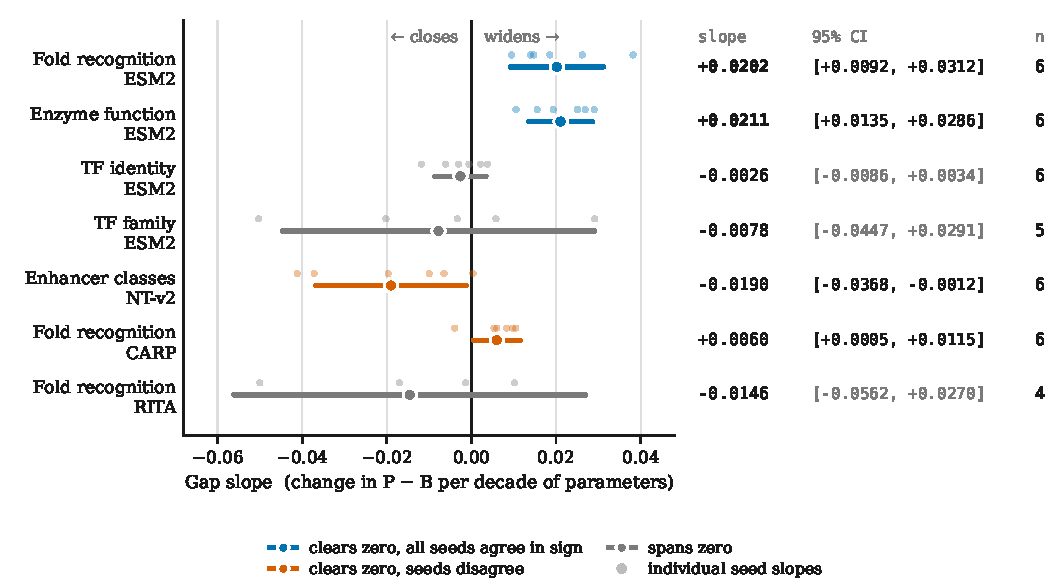
\includegraphics[width=\textwidth]{figures/gap_forest.pdf}
\caption{Per-seed slopes of the elicitation gap on $\log_{10}$(parameters), fitted
one slope per seed and averaged across seeds with a Student-$t$ interval. Small
dots are individual seed slopes. Only two rows both clear zero and agree in sign
across every seed.}
\label{fig:forest}
\end{figure}

\begin{table}[h]
\centering
\small
\begin{tabular}{@{}llrrcl@{}}
\toprule
\textbf{task} & \textbf{family} & \textbf{seeds} & \textbf{mean slope/decade} &
\textbf{95\% CI} & \textbf{seeds agreeing} \\
\midrule
fold recognition & ESM2 & 6 & $\mathbf{+0.0202}$ & $[+0.0092, +0.0312]$ & 6 of 6 \\
enzyme function & ESM2 & 6 & $\mathbf{+0.0211}$ & $[+0.0135, +0.0286]$ & 6 of 6 \\
TF identity & ESM2 & 6 & $-0.0026$ & $[-0.0086, +0.0034]$ & disagree \\
TF family & ESM2 & 5 & $-0.0078$ & $[-0.0447, +0.0291]$ & disagree \\
enhancer classes & NT-v2 & 6 & $-0.0190$ & $[-0.0368, -0.0012]$ & disagree \\
\bottomrule
\end{tabular}
\caption{Elicitation-gap slopes per decade of parameters
(\texttt{analyse\_family\_gap.py}).}
\label{tab:gap}
\end{table}

Table~\ref{tab:gap} and Figure~\ref{fig:forest} give the per-seed slopes.
Two tasks widen, clearly and reproducibly. Fold recognition and enzyme function
share no data, no label space and no split procedure, and all twelve of their
seeds are positive. \textbf{These are the strongest results we have.} Their means
differ by 0.0009, but we do not read that agreement as evidence of a shared
constant: the twelve individual seed slopes span $+0.006$ to $+0.040$, a factor of
seven, so the closeness of the two means is within their own sampling noise. The
two also share seed indices and are correlated across paired seeds ($r = 0.59$),
so they are two tasks and not two independent experiments.

Two tasks show nothing, and \textbf{both are ceiling-compressed} --- TF identity
has 0.11 of room and TF family 0.19, against 0.51 and 0.63 for the two that
widen. A gap cannot open where the behavioural score is already near the maximum,
so these two nulls are consistent with ceiling artefacts rather than with an
absence of the effect. We cannot distinguish those possibilities with this design.

The genome task points the other way, and its interval clears zero by 0.0012
while its seeds disagree in sign. \textbf{We report it as weak.} It has as much
room to improve (0.51) as fold recognition (0.51), so headroom does not explain
that difference; modality, architecture and family remain confounded, and this
design cannot separate them. Its ladder is also the shortest here at 0.96 decades.

\textbf{The widening is therefore not a general property of biological foundation
models.} Any claim that it is would overreach the evidence.

\subsection{A second and a third model family}

Fifty of our sixty-nine protein cards, before CARP was added, were ESM2 ---
forty-two trained checkpoints and eight randomly-initialised control arms. To test
whether the finding is a property of one lab's recipe we added
CARP~\citep{yang2024carp}: four sizes over 3.02 decades, one training set, one
objective, and a dilated-convolutional architecture rather than a transformer.

\begin{table}[h]
\centering
\small
\begin{tabular}{@{}lrrrcl@{}}
\toprule
\textbf{family} & \textbf{span} & \textbf{seeds} & \textbf{mean slope/decade} &
\textbf{95\% CI} & \textbf{seeds agreeing} \\
\midrule
ESM2 & 2.57 dec & 6 & $+0.0202$ & $[+0.0092, +0.0312]$ & 6 of 6 \\
CARP & 3.02 dec & 6 & $+0.0060$ & $[+0.0005, +0.0115]$ & 5 of 6 \\
RITA & 1.15 dec & 4 & $-0.0146$ & $[-0.0562, +0.0270]$ & disagree \\
\bottomrule
\end{tabular}
\caption{Fold recognition across three model families.}
\label{tab:families}
\end{table}

Table~\ref{tab:families} sets the three families side by side. CARP agrees in
direction and not in magnitude: a third the size, a lower bound
clearing zero by 0.0005, one dissenting seed. We report this as \textbf{weak
corroboration, not confirmation}.

An incidental observation may matter more. CARP's per-rung gaps are about four
times smaller than ESM2's in absolute terms (mean $|$gap$|$ 0.011 against 0.044)
and every CARP rung's six-seed interval straddles zero, while every ESM2 rung's
clears it. And CARP-640M scores higher than ESM2-3B behaviourally in five of six
seeds (mean $+0.029$, 95\% CI $[-0.003, +0.061]$) with a fifth of the parameters
--- an interval that spans zero, so we claim comparable performance and not
superiority. Two strong families, comparable performance, several-fold different
in how much their internals hold back. If this holds, the elicitation gap is at
least as much a fact about architecture as about scale. No single-family study
could have seen it.

Within CARP we can ask whether width or depth carries this, because its rungs vary
the two separately. Paired within-seed contrasts do not resolve it: width alone
($\times 8$ width, equal depth) gives $+0.0019$ $[-0.0219, +0.0257]$ and depth
alone ($\times 2$ depth, equal width) gives $+0.0106$ $[-0.0070, +0.0283]$, both
spanning zero. We report the question as open rather than answered.

\paragraph{A note on availability.} We surveyed roughly thirty candidate families
to find one second ladder. Almost nothing is built to be a scale ladder:
ProGen2~\citep{nijkamp2023progen2} gives its top rung twice the tokens; families
change their data mixture at the top; Geneformer~\citep{theodoris2023geneformer}
crosses a training generation between rungs; most families span under 1.5 decades.
\textbf{The scarcity of clean scale ladders is itself a finding}, and scaling
claims in this literature inherit it whether or not their authors say so.

\subsection{Recoverability under light fine-tuning}

\begin{table}[h]
\centering
\small
\begin{tabular}{@{}lrcl@{}}
\toprule
\textbf{task} & \textbf{mean slope/decade} & \textbf{95\% CI} &
\textbf{seeds agreeing} \\
\midrule
fold recognition & $+0.0203$ & $[+0.0076, +0.0330]$ & 6 of 6 \\
enzyme function & $+0.0238$ & $[+0.0143, +0.0333]$ & 6 of 6 \\
\bottomrule
\end{tabular}
\caption{How much light fine-tuning adds over the model's own output
(F\,$-$\,B), six seeds each.}
\label{tab:recov}
\end{table}

Table~\ref{tab:recov} gives the slopes: twelve seeds of twelve positive, on
two tasks. The two task means differ by
0.0035, which is within their own sampling noise rather than evidence of a shared
constant; individual seed slopes span $+0.006$ to $+0.040$. The two tasks share
seed indices and are correlated, so they are not independent replications.

\textbf{This result is confounded by construction}, and we flagged it as
unpublishable for weeks on that basis: every rung receives an identical 400-step
budget while the largest model has 375 times the parameters of the smallest, so
``a fixed budget is worth more to a bigger model'' predicts exactly this. The
iso-performance measurement of Section~\ref{sec:isomethod} was built to remove
that confound, and is reported next.

\subsection{Budget required to reach a fixed capability}

Applying the iso-performance measurement of Section~\ref{sec:isomethod} at three
target scores gives the slopes in Table~\ref{tab:cost} and the fits in
Figure~\ref{fig:cost}.

\begin{figure}[t]
\centering
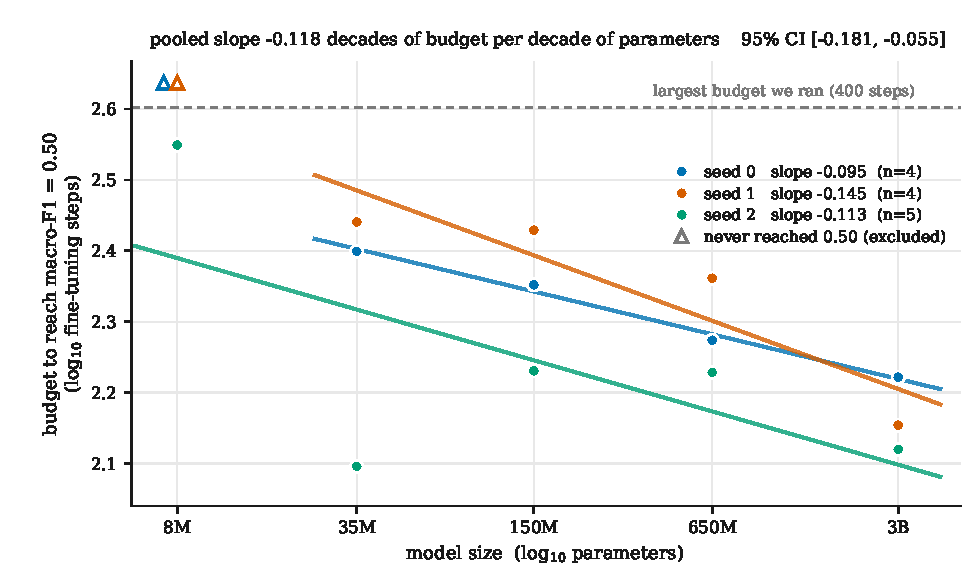
\includegraphics[width=0.92\textwidth]{figures/cost_scaling.pdf}
\caption{Budget required to reach a fixed macro-F1 of 0.50, against model size.
Each point is one model in one seed, and each budget is a separate fine-tuning run
annealed to its own endpoint. The dashed line marks the largest budget we ran, 400
steps. The two open triangles above it are the seeds in which the smallest model
(8M) never reached 0.50 within that budget: for those seeds no crossing point
exists, so that model cannot be placed on the vertical axis and is left out of the
fit. This is why seeds 0 and 1 are fitted on four rungs and seed 2 --- whose 8M
model did reach the target, at about 354 of 400 steps --- on five.}
\label{fig:cost}
\end{figure}

\begin{table}[h]
\centering
\small
\begin{tabular}{@{}lrc@{}}
\toprule
\textbf{target score} & \textbf{mean slope (decades budget / decade params)} &
\textbf{95\% CI} \\
\midrule
0.40 & $-0.040$ & $[-0.096, +0.016]$ \\
0.45 & $-0.094$ & $[-0.265, +0.078]$ \\
\textbf{0.50} & $\mathbf{-0.118}$ & $\mathbf{[-0.181, -0.055]}$ \\
\bottomrule
\end{tabular}
\caption{Iso-performance cost scaling, pooled over three seeds.}
\label{tab:cost}
\end{table}

All nine seed-by-target slopes are negative. At the hardest target the pooled
interval clears zero and all three seeds agree in sign: \textbf{a tenfold larger
model reaches the same score on roughly 0.76 of the budget.}

Three fragilities belong with that number, none of them visible in the table. No
individual seed's own fit clears zero except the first. The pooled interval spans
zero if any single seed is dropped --- three seeds is the minimum this estimator
can speak from, not a comfortable margin. And the smallest rung is censored at
this target in two of three seeds but not the third, where it crosses at about 354
of 400 steps; the result depends on that asymmetry, and dropping the smallest rung
uniformly across seeds would change it.

This measurement does not carry the fixed-budget confound of the preceding
subsection. Two measurements
--- one confounded, one not --- point the same way, which is what makes the
recoverability result interpretable rather than merely suggestive.

The effect appears only where the target is hard enough to separate models. At
easier targets every model arrives quickly and the direction, while consistent, is
not distinguishable from zero. That is a coherent result rather than a null:
capabilities that are cheap for everyone cost roughly the same for everyone.

\subsection{Single runs do not survive replication}
\label{sec:repl}

\begin{figure}[t]
\centering
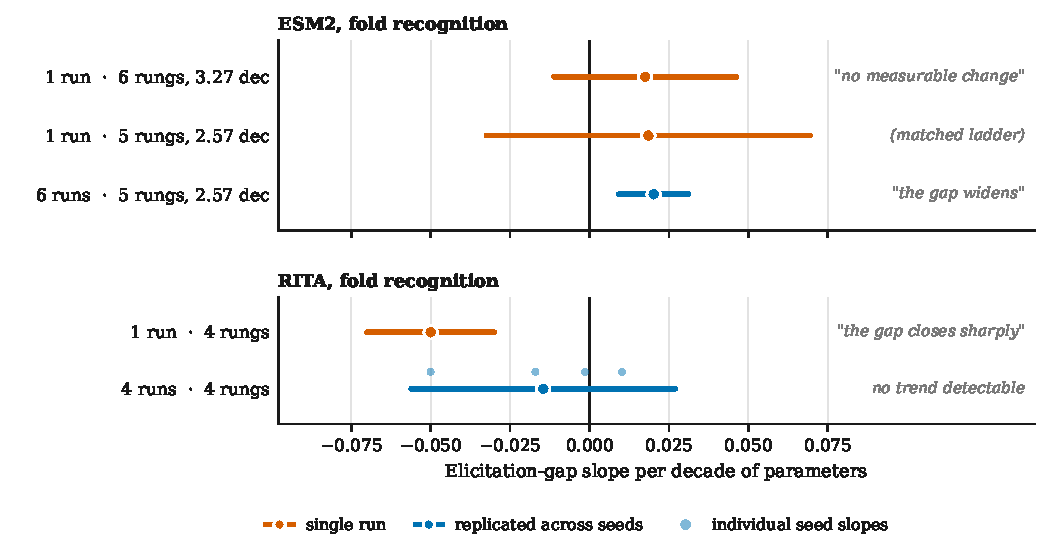
\includegraphics[width=\textwidth]{figures/replication.pdf}
\caption{The same quantity, measured once and measured repeatedly. For ESM2 the
point estimate barely moves while the interval collapses; for RITA a single run
produced an effect clear of zero that four runs erase.}
\label{fig:repl}
\end{figure}

Our own headline reversed (Table~\ref{tab:repl}, Figure~\ref{fig:repl}):

\begin{table}[h]
\centering
\small
\begin{tabular}{@{}llrcl@{}}
\toprule
\textbf{evidence} & \textbf{ladder} & \textbf{slope} & \textbf{95\% CI} &
\textbf{what we concluded} \\
\midrule
1 run of fold recognition & 6 rungs, 3.27 dec & $+0.018$ & $[-0.011, +0.046]$ &
``no measurable change'' \\
1 run, matched ladder & 5 rungs, 2.57 dec & $+0.019$ & $[-0.032, +0.069]$ & --- \\
6 runs of fold recognition & 5 rungs, 2.57 dec & $+0.020$ & $[+0.009, +0.031]$ &
the gap widens \\
\bottomrule
\end{tabular}
\caption{One quantity, measured once and measured six times. The middle row is
the like-for-like comparison: the same ladder, read once and read six times.}
\label{tab:repl}
\end{table}

The middle row is the like-for-like comparison, and it makes the point more
sharply than the one we published: on the same ladder, one run gives an interval
4.6 times wider than six runs, around an almost identical estimate.

\textbf{The measurement barely moved. Only the uncertainty did.} The first number
was a statement about how little we had run, dressed as a statement about models.
We had published it.

It reverses in the other direction too. RITA appeared on a single run to show the
gap closing sharply ($-0.050$, interval clear of zero, four nearly-collinear
points). Four seeds gave $-0.050$, $-0.001$, $-0.017$, $+0.010$: mean $-0.015$,
interval spanning zero, seeds disagreeing in sign. The apparent effect was one
seed.

The same pattern recurred at least six times, on two quantities --- the gap and
recoverability --- across fold recognition, enzyme function, enhancer
classification, CARP and RITA. In the ESM2 headline case the estimate barely
moved and only the interval did; in the RITA case the estimate itself collapsed to
under a third of its single-run value. Both are failures of a single run, by
different mechanisms.

The honest form of the claim is narrower than the one we first wrote.
\textbf{Every single-run result in this programme that we treated as a finding
changed its verdict under replication.} The single-run results that survived
unchanged were nulls on tasks that are still nulls --- which is not reassurance,
since a null is what an underpowered design returns by default.

The generalisation is uncomfortable and we state it plainly. Comparable papers in
this subfield report either no interval at all or a best-minus-worst spread over
about three runs, across four to six model
sizes~\citep{gao2025pfmbench,xu2022peer,jamasb2024proteinworkshop}. Three runs is precisely the count that read as a null here before
six runs reversed it. The problem is not confined to this subfield: across 485
models and more than a thousand fitted laws, scaling-law estimates are noisy and
sensitive to which runs enter the fit~\citep{choshen2024hitchhiker}.
A four- or five-point ladder read once has two or three residual degrees of
freedom and an interval wide enough to contain almost anything. ``Contains zero''
is not ``is zero''.

\section{Discussion}

\subsection{Scope of the claims}

Several claims are \emph{not} supported by this design, and we set them out
explicitly. We do not claim:

\begin{itemize}
\itemsep2pt
\item \textbf{That the gap widens generally.} It widens on two tasks of five. The
distinguishing factor is not identified.
\item \textbf{That this is about scale rather than architecture.} CARP's gaps are
several-fold smaller than ESM2's at comparable performance.
\item \textbf{That four or five checkpoints are a sample of protein language
models.} Our intervals reflect seed noise, not model-sampling noise. Strictly,
each result is about those checkpoints.
\item \textbf{Anything about single-cell models.} They have no clean scale ladder.
\item \textbf{That the cost result holds at easy targets.} It does not.
\end{itemize}

\subsection{Measurement defects and the direction of their bias}
\label{sec:defects}

The full taxonomy is given in the supplementary material; eight load-bearing ones
are given here. We report the classification rather than a tidy count, because
the count is the sort of thing this paper is about: of the defects that biased a number at all,
\textbf{every one biased it in our favour}. The remainder destroyed or corrupted
work without pointing in a direction --- a failed deploy, an unpinned dependency,
a dead parameter. We do not think this asymmetry is luck. \textbf{A pipeline is
built by people who want it to work, so errors whose output looks like success
survive review, and errors whose output looks like failure get chased down the
same afternoon.}

The load-bearing ones:

\begin{enumerate}
\itemsep3pt
\item \textbf{The probe layer was chosen by argmax on the test set.} On the model
where we isolated it (TF identity, ESM2-650M) the honest validation-selected gap
is $+0.0016$ and the test-selected one $+0.0188$ --- a twelvefold inflation, of
which $\sim$92\% of the apparent gap was selection bias. The fix for it left the
same bug on its fallback branch.
\item \textbf{An interval that covered 90\% while claiming 95\%}, which retracted
the only trend we had then called significant.
\item \textbf{A scaling slope fitted over rungs that failed their own null test}
--- the $p$-values were computed by our pipeline, written to the cards, and loaded
back by the function doing the fitting, which never read them.
\item \textbf{A missing rung was not missing at random.} An out-of-memory error
kills the \emph{largest} model, and the top of a ladder is where a plateau
masquerading as a trend gets caught. Recovering one such rung turned $+0.084$
$[+0.030, +0.138]$ into $+0.040$ spanning zero.
\item \textbf{Quantisation reported as an effect.} A budget ratio of exactly 1.00
and a slope of exactly 0.000 were the measuring grid, not the models. \emph{A
suspiciously round number is an artefact until shown otherwise.}
\item \textbf{A gap of exactly zero because no layer could be chosen} is not a gap
of zero. Where a split left too little to carve a validation set, the probe fell
back to the sanctioned surface and P equalled B identically --- a number that
looks like a measurement and is a statement about the instrument.
\item \textbf{The measurement built to remove a confound contained one.}
Steps-to-target read off a single annealed trajectory is biased, and not even with
a constant sign.
\item \textbf{Untrained control arms were regressed as if they were models.} Four
randomly-initialised ESM2 checkpoints sat inside the ladder on both
transcription-factor tasks, at the same parameter counts as their trained twins,
silently doubling four of five rungs. This one was found by the adversarial check
on \emph{this paper}, after the results in it had been written up. Correcting it
did not change any verdict, which is luck rather than vindication.
\end{enumerate}

\subsection{Limitations}
\label{sec:lim}

\paragraph{Model-sampling noise is not represented.} Our intervals come from
repeated runs on fixed checkpoints. With five checkpoints per family, the
population of models is not sampled and cannot be.

\paragraph{Single-cell is out of scope, for a structural reason.} Those tasks run
one real model plus two non-model comparators. The obvious remedy fails:
Geneformer's three sizes cross a training generation (V1$\rightarrow$V2), which is
the confound that disqualified other candidates, and V2 alone spans 0.48 decades.
No published single-cell ladder holds its recipe fixed.

\paragraph{TF family contributes five usable seeds of six.} Its split drops five
to eight of fourteen classes depending on seed (seven in four of six), and under
one seed too little remained to carve a validation set, so every rung fell back to
the sanctioned surface and the whole seed was excluded. The surviving seeds are
therefore not a random subset --- they are the ones whose inner validation carve
retained more than one class. Which way that biases the slope is not established:
the excluded seed is middling on class-drop count, so ``easier split'' is a
description we cannot support. More seeds does not fix the selection.

\paragraph{The cost measurement censors its smallest rung} at the hardest target,
in two of three seeds, leaving four rungs there and five in the third --- where
that model does reach the target, at about 354 of 400 steps. So it sits at the
grid ceiling rather than beyond it, and the ``conservative exclusion'' argument
holds only conditionally: including it steepens the slope if its true cost exceeds
roughly 290 steps in the first seed and 380 in the second, and flattens the slope
below those thresholds.

\paragraph{Three seeds on the cost measurement is thin.} Only its hardest target
clears zero, and the pooled interval spans zero if any one seed is removed.

\paragraph{We examined three targets and report one as significant.} They are not
independent --- all three are derived from the same evaluated curves --- but the
multiplicity is real, and choosing 0.50 as the headline after seeing all three is
a forking path we did not pre-register.

\section{Conclusion}

The empirical results are real, reproducible, and narrower than we would like.
Two tasks widen; one measurement free of the obvious confound agrees.

The methodological result is, we think, the more useful contribution. It is
cheaply actionable --- repeat your runs --- it is verifiable against our own
published reversals, and it applies to a literature that mostly does not do it. We
would rather be the paper that says ``our headline reversed, here is the
arithmetic'' than one more single-run scaling curve.


\section*{Key Points}
\begin{itemize}
\itemsep2pt
\item Reading a model's sanctioned output and a linear probe of its best internal
layer \emph{at identical readout capacity} makes the difference between them a
property of the model rather than of the probe.
\item The elicitation gap widens with scale on two of five tasks, is undetectable
on two ceiling-compressed tasks, and reverses on a genome task; a second
architecture shows gaps several-fold smaller at comparable performance, so
scaling behaviour here is task- and architecture-dependent rather than lawful.
\item Holding the score fixed and measuring the budget required removes the
confound that a fixed fine-tuning budget is worth more to a larger model; that
budget falls by roughly a quarter per decade of parameters.
\item Single-run scaling claims in this literature are unreliable in both
directions: our own published headline reversed under replication, with the point
estimate almost unchanged and only the interval narrowing.
\item Of twenty-nine measurement defects found in our own pipeline, every one of
the twenty-six that biased a number biased it in our favour --- an asymmetry we
argue is structural rather than incidental.
\end{itemize}

\section*{Data availability}

\begin{sloppypar}
All result cards, sweep files and analysis code underlying every number in this
paper are openly available at \url{https://github.com/Biodyn-AI/probe-scaling},
and archived at \doi{10.5281/zenodo.22061975}~\citep{kendiukhov2026code}. Result cards are under
\texttt{data/cards/}; iso-performance sweeps under \texttt{data/sweeps/}. The analysis scripts, figure-generation script and bibliography generator in
that repository regenerate every figure, table and reference in this paper from
those files, and its test suite re-derives each published value and fails if it
moves. Reproducing the paper requires neither a GPU nor model weights: the
released cards are the input. No new experimental data were generated; all model checkpoints and
benchmark datasets are third-party and cited at first use.
\end{sloppypar}

\section*{Funding}

This work was supported by Pivotal Research.

\section*{Declaration of generative AI use}

This declaration follows the ISCB acceptable-use policy for large language models.

A large language model (Claude, Anthropic) was used as a coding and checking
assistant in the computational work, under the author's direction and review, in
the following ways. It assisted in writing and refactoring the evaluation
harness, the analysis functions and the figure-generation code, all of which are
released in the repository named under Data availability and are covered by the
test suite. It was used as an evaluation technique in the sense the policy
describes --- to search the pipeline for inconsistencies and anomalies --- which
is how a number of the measurement defects reported in Section~\ref{sec:defects}
were surfaced. It was used to retrieve and verify bibliographic metadata: every
reference in this paper was resolved programmatically against doi.org or the
arXiv API by the script \texttt{build\_bib.py}, which fails rather than emit an
unresolvable entry. It also assisted in preparing the \LaTeX{} sources of the
tables and figures.

All outputs of the assistant were reviewed by the author, and every numerical result
reported here was re-derived from the released result cards by the analysis
scripts in the repository named under Data availability.


\bibliographystyle{plainnat}
\bibliography{refs}

\end{document}
